\section {Goals}
\label{sec:goals}
Content Profiling is a topic that combines two important parts of digital preservation and acts as the glueware, that holds up a digital preservation system in terms of its integrity. On the one side, there are lower level technical procesess, such as characterization, which play an important role not only to preservation planning but to DP in general. These procesess have to deal with single objects (even though the scale can be very large). As output they provide information to quality assurance activities and workflows as well as preservation planning. The identity and meta data extracted out of every single digital object is the scaffold that enables many other processes and applications to do their work. Consequently, the tools that provide this data care the responsibility for any subsequent process that relies on this data and its validity.
On the other side, there is preservation planning, which is a higher level process that deals with sets of objects. As such, preservation planning deals with a great deal of data, but is responsible that every single object complies to the requirements of a preservation expert after a preservation action is conducted. The usual size of real world-scenario collection (or set of objetcts) does not allow the test and inspection of every single object before and after each evaluated preservation action. Thus, a bigger picture of the content at hand plays an immense role in the choosing of representative samples and implicitly on the decision made by a preservation expert.

In order to ensure that these two different important parts of Digital Preservation fit together and provide a valid and effective outcome, an adaptor is needed. It has to transform the fine granular output of one process into an aggregated higher level input to the other.

Identification and characterizaion are technical processes that can be conducted in automated fashion. Preservation Planning on the other hand is a process, that can be automated only to a certain extent and will always rely on a human decision. Nonetheless, the degree of automation can be highly improved as the current state of the art is. All this outlines the goals of the content profiling process, which are summarized as follows:

\begin{itemize}
\item Enable automatic and scalable aggregation of meta data provided by identification and characterization tools.
\item Create a well-defined, machine readable footprint of the content at hand.
\item Enable planning experts to analyse and filter content into homogeneous parts, based on different characteristics of the content that make sense from use case to use case.
\end{itemize}
% goals

\section{Preservation Planning}
The preservation planning process is a well-defined workflow consisting of three phases with several steps amounting to 11 altogether \cite{STR07_jcdl}. The process specification was created during the PLANETS project and has been verfied by numerous case studies since then. 

In the first phase, \textit{``Define Requirements''}, the scope of the preservation plan is demarcated. The preservation expert has to follow three steps; to provide information about the collection, environment etc. (\textbf{Define Basis}), to choose representative sample records for experimentation (\textbf{Define Sample Records}) and to identify the requirements for the preservation plan or the so called objective tree, which summarized high-level goals of the plan (\textbf{Identify Requirements}). 

In the second phase, \textit{``Evaluate Alternatives''}, another 5 steps have to be followed. Starting with the definition of alternatives (\textbf{Define Alternatives}), the responsible preservation expert has to choose a set of potential actions, with all related informations, such as environment, tool invocation parameters, etc. In the following (\textbf{GO/NO-GO}) step a decisions is made whether to proceed or not based on each preservation action, the estimated resources and the defined requirements. After that the planner has to create suitable experiments (\textbf{Develop Experiment}), which are well-documented, repeatable set of actions with their environment and the capability to capture their results. In the following (\textbf{Run Experiment}) step, each preservation action is executed against the chosen sample records in order to obtain different results. In the last step of this phase (\textbf{Evaluate Results}) the results of the experiment output is evaluated against the objective tree in order to check if the identified requirements were met or not.

The third phase, \textit{``Consider Results''}, is responsible for the objective analysis of the results. In its first step (\textbf{Transformed Measured Value}) all experiment results are transformed into the same scale (0-5) making use of special transformation tables and utility function. The following (\textbf{Set Importance Factor}) step provides the ability to equal the weight of different parts of the requirement objective tree as not all goals are equally important. In the last step (\textbf{Analyse Results}) all measures are aggregated per objective and provide the planner with a preservation action recommendation and the necessary basis for a decision.

\begin{figure}[htb]
\begin{center}
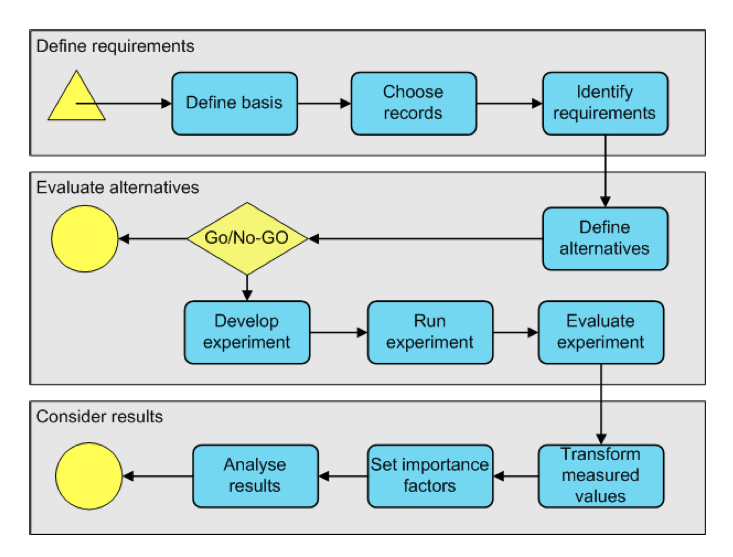
\includegraphics[width=4.5in]{figures/contentprofiling/planningworkflow.png}
\caption{Overview of PLANETS Preservation Planning workflow \cite{Becker:2008:PSO:1378889.1378954}.}
\label{fig:planningworkflow}
\end{center}
\end{figure}

The workflow is depicted in figure \ref{fig:planningworkflow} and provides the current state of the art in preservation planning matters. Although it provides a very solid theoretical ground and a complete specification that is working in practice, there is one flaw in the concept, which leaves space for huge errors caused by human inconpetence, lack of knowledge and understanding of the collection or even sloppiness.

As one can see from the workflow all the results strongly depend on the defined goals and the analysis of the experiments output. We assume that a preservation expert will understand the objectives of his organization. Since the identification of requirementes and the setting of the goals and objectives are very important steps that are also strongly dependent on the organizational background of the preservation expert, we also assume that it is unlikely they will cause errors and misunderstandings in later steps. Also if the planner happens to choose wrong preservation action alternatives, the result will be in the worst case scenario a 'Do Nothing' alternative, which will not solve the problem at hand, but will also not do any damages.
However, there is one step that could have serious implications and even cause damage or resource loss if taken lightly. Consider the following example, where the chosen sample records are picked up at random from a medium sized collection with several thousands of objects. Then the experiments show a particular preservation action is very feasible and the planner chooses to execute this action over the whole content, due to the experiments output and the consequent analysis. Although the analysis, and the decision are perfectly valid (in their implementation and execution), it could turn out that the result of the preservation operation does not meet the requirements defined. This could happen, due to many different aspects in the format and content profile of the collection at hand. To summarize, the defined requirements and objectives are ok, the experiments are valid, the analysis is correct, but the overall results are not feasible due to the false premise, that the random chosen set of sample records is representative. Damage could be done, if there is no reasonable and thorough quality assurance process afterwards. This work tries to prevent the described problem by reducing the bias of the experiments. This is to be achieved by thorough analysis and automatic representative selection in the early steps of the workflow.

One can argue, that no real preservation expert will choose representatives at random. Although, this might be true, there are numerous other factors that have to be considered when choosing the representatives and since the collections that are worth preserving are often big enough, the overhead for the preservation expert is just not feasible to select them by hand. Thus the representatives are usually chosen by format and format version in combination with their size (minimum, maximum and average).

Note, that there is a fourth phase (\textit{``Build preservation plann``}) which adds an important part to the workflow and results in an applicable real world preservation plan artifact. The planning tool PLATO, developed at the University of Technology in Vienna, implements this process and appends a fourth phase, where the user/planning expert can create an executable plan, which can be deployed within a repository. The preservation action plan is a well defined specification that serves the purpose of documentation of the decisiion and contains the executable part, which specifies the tools, environment and parameters to use during the preservation operation.

However, in its current release, the planning tool supports only manual sample records definition. Although it assists the planner with integrated characterization tools, it cannot provide higher certainty in the validity of the chosen representatives. Integration with another tool that provides a complete content profile (generated in an automatic fashion) would provide a huge benefit to preservation planners.

\section{Collection \& Content Profiling}
\label{sec:content_profiling}
TBD
% what is it c3
% jhove (identify, characterize, validate)
\subsection{The content profiling process}
Content profiling consists of three main parts; data harvesting, data aggregation and analysis.

The first part is responsible for parsing the output of the meta data and adapting it to the internal model of the profile tool. Here, special post-processing steps can be applied to each meta data object in order to refine the data. For example, if the tool provides unnormalized data, special actions can be provided, or if there are conflicted values of the same property provided by different sources, data cleanup actions and rules can be executed. These post-processing steps can have huge impact on the final result and thus should not be executed lightly, but only through special configuration steps, done by preservation experts, that understand the source of the meta data, the operations of the identification and characterization tools and the implications of such alterations of the data. Thus, such functionality of the content profiler has to be done in a flexible fashion and has to allow special the configuration that can alter and turn on and off such behavior.

The second step can be done either after the data is parsed, normalized and stored or on demand if the underlying data store provides the necessary facilities. It is responsible to present the big picture of the data in a smaller footprint and structured form, so that other programms and tools can integrate with it. It should provide enough flexibility to understand the data but also a smaller footprint.

The third step is more of a high level feature, that has to be conducted mostly manually by the preservation expert. This means that it will rely on specific desicions and will need the input of a user. Nonetheless it should be automated as much as possible and shall support the user in her decisions.


\subsection{Data \& Normalization}
In order to achieve the goals outlined above, the meta data provided by the characterization tools has to be normalized and should fit into a unified model no matter its origin. For this purpose, a simple but flexible domain model has to be created that allows, properties, their measures, provenance information and more to be stored at one place.
The data structure has to enable efficient aggregation and querying of the data. 

Another important aspect of the data is its validity. Obviously if the data that is provided is valid and of high quality, then the created profiles and the chosen representative sample objects will solely rely on the processes and algorithms involved. If these processes and algorithms are validated and on their terms of high quality, then the result will be a profile that enables unbiased experiments in preservation planning activities. As profiling depends on the meta data and the tools that are able to extract it, it is of great importance that quality assurance is conducted. Unfortunately, the state of the art does not provide many methods of checking the validity of a characterization tool. %cite? qa in characterization?
% why is it important (iteration of before)

\subsection{Format}
% specification (representation, xml, rdf)
There are numerous ways of representing such a profile. However, from the observations of the previous chapter there are number of goals that it has to fulfill.
It has to follow a well-defined schema; the profile has to be in a structured, machine readable form as it will act as input to other information systems in the DP landscape.
Obviously, it has to aggregate the raw data but still provide enough insight into the content at hand. The profile should be able to separate the content based on different characteristics. Here it is important that a user or a user application is able to go one step back and examine the filtering criteria. Finally, the profile should include a small set of representative objects, with their full characteristics and a way to identify all objects in a set or collection that fit into the specified filter. The latter could be done, either via some kind of query or just by a list of objects outlines the identifiers of all selected objects.

\subsection{Integration with DP Systems}
% integration with other tools, such as repositories and planning tools
A content profiler tool can provide benefit to numerous systems and users in a Digital Preservation environment. On the one hand it can act as direct input to Preservation Planning and can spare a planning expert a lot of time defining and outlining a plan. 

On the other hand it supplies the needed facilities to analyse new content ingested within a repository and can act as input to monitoring systems, that can raise alerts if certain problems are detected. For example, an organization should have a policy that defines, which objects have to be preserved and one that defines how many objects of a certain type can exist without a valid plan associated to them. Now consider that each day a great deal of new objects is ingested into the repository of that particular organization. By the end of a certain time period a content prifle is regenerated and a monitoring system obtains and reevaluates this result agains the organizational policies. It will be fairly easy to detect a potential threat and to notify the involved stakeholders and actors in order to resolve it, provided all of these pieces of the puzzle fit together.

Another great deal of the combination of such a content profile and monitoring system can be a global content profile. If enough organizations, such as Web Archives, Libraries, etc. are willing to share the profiles (or parts of them) they have with such a central monitor, the result will most probably be a representative overview of the global state of the world \cite{duretec:2012:watch}. Valuable information, such as the number of formats used within a certain domain, the preferred type of files within a user community, the emergence of new file formats, the decline of old file formats and much more can be detected. Provided that enough content-holding institutions are ready to sacrifice a bit of their privacy, the mutual benefit could be something much more valuable.

\section{Representative Sets}
\label{sec:representative_sets}
% what is the problem,
% how do we create them/find them


\section{Continuos Profiling}
